\begin{frame}{Discrete choice models}
  \begin{columns}
    \begin{column}{0.65\textwidth}
      \begin{itemize}
        \item Linear regression is great, but how do we predict a discrete choice?
        \item For example, the choice of car or bus?
      \end{itemize}
    \end{column}~%
    \begin{column}{0.34\textwidth}
      \includegraphics[width=\textwidth]{img/hfx.jpg}
    \end{column}
  \end{columns}
\end{frame}

\begin{frame}{Applications of discrete choice models}
  \begin{itemize}
    \item Mode choice
    \item Destination choice
    \item Route choice
    \item Residential location choice
    \item Vehicle choice
  \end{itemize}
\end{frame}

\begin{frame}{Measurement levels}
  \begin{itemize}
    \item Nominal: \pause categories with no order (e.g. colors)
    \pause\item Ordinal: \pause ordered categories with no information about distance between them (e.g. much less, less, same, more, much more)
    \only<5-8>{\item Interval:~} \only<6-8>{distances between items are meaningful, ratios are not (no meaningful zero; e.g. temperature)}
    \only<7-8>{\item Ratio:~}\only<8>{distances between items and ratios are meaningful (e.g. income)}
    \only<9>{
      \textcolor{gray}{
        \item Interval:~distances between items are meaningful, ratios are not (no meaningful zero; e.g. temperature)
        \item Ratio:~distances between items and ratios are meaningful (e.g. income)
      }
    }
  \end{itemize}
\end{frame}

\begin{frame}{Binary outcomes}
  \begin{itemize}
    \item Simpler case is a binary outcome
    \item To bike or not to bike
    \item To carpool or not to carpool
    \item ...and so on
  \end{itemize}
\end{frame}

\begin{frame}{One option: the linear probability model}
    \begin{itemize}
      \item Uses linear regression to predict binary outcome
      \item Code outcomes as 0 or 1
      \item Interpret coefficients as change in probability
    \end{itemize}
\end{frame}

\begin{frame}{One option: the linear probability model}
  \centering\begin{tabular}{lrrrrrr}
  \toprule
  {} &  Coefficient &  Std. err. &  $t$-value &  $p$-value &  95\% Conf. &   Int. \\
  \midrule
  Constant        &        0.535 &      0.012 &     43.622 &        0.0 &      0.511 &  0.559 \\
  Cars per driver &       -0.042 &      0.009 &     -4.540 &        0.0 &     -0.061 & -0.024 \\
  \bottomrule
  \end{tabular}
  \begin{tabular}{lclc}
  Dependent variable & \multicolumn{3}{l}{Carpool on trip} \\
  $R^2$ & 0.00 & Adjusted $R^2$ & 0.00 \\
  Sample size & 10000 && \\
  \end{tabular}\\
  \tiny\citenhts
\end{frame}

\begin{frame}{One option: the linear probability model}
  \centering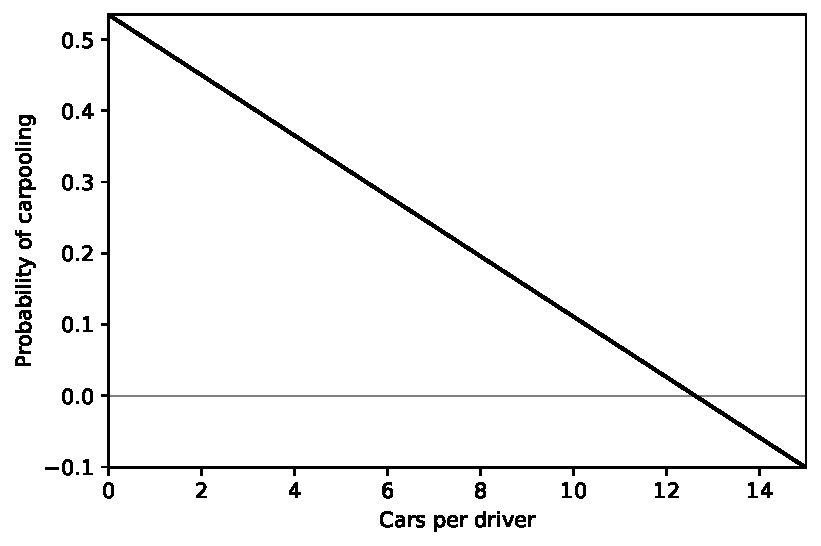
\includegraphics[width=0.7\textwidth]{fig/linearprobabilitymodel.pdf}\\
  \tiny\citenhts
\end{frame}

\begin{frame}{One option: the linear probability model}
  \centering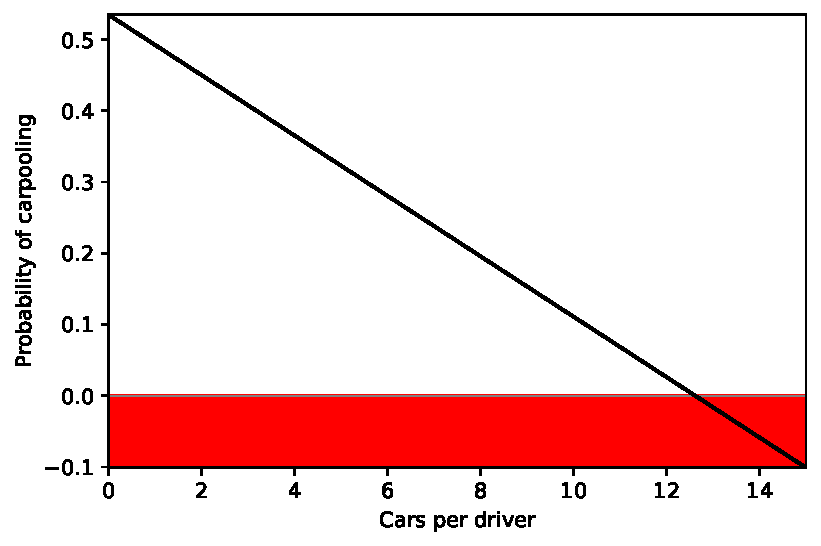
\includegraphics[width=0.7\textwidth]{fig/linearprobabilitymodel_highlight.pdf}\\
  \tiny\citenhts
\end{frame}

\begin{frame}{Alternate option: random utility models}
  \begin{itemize}
    \item Assume that the probability of choosing an option is a function of \emph{utility}
    \item Utility is a concept from economics, basically means value
    \item Utility is usually a linear function---like linear regression!
    \item A transformation is applied to utility to model probability
    \item Utility is a \emph{latent variable}---we don't measure it, we infer it
  \end{itemize}
\end{frame}

\begin{frame}{Alternate option: random utility models}
  \begin{tikzpicture}
    \node[draw=black,inner sep=5pt,anchor=west] (v1) at (0, 7) { Variable 1 };
    \node[draw=black,inner sep=5pt,anchor=west] (v2) at (0, 5) { Variable 2 };
    \node[draw=black,inner sep=5pt,anchor=west] (v3) at (0, 3) { Variable 3 };
    \node[draw=black,inner sep=5pt,anchor=west] (carpool) at (7, 5) { Probability of carpool };

    \only<1>{
      \draw[->] (v1.east) -- ([yshift=3pt] carpool.west);
      \draw[->] (v2.east) -- (carpool.west);
      \draw[->] (v3.east) -- ([yshift=-3pt] carpool.west);
    }

    \only<2-3>{
      \node[draw=black,inner sep=5pt,rounded corners=0.2cm,anchor=west] (utility) at (5, 5) { Utility };
      \draw[->] (v1.east) -- ([yshift=3pt] utility.west);
      \draw[->] (v2.east) -- (utility.west);
      \draw[->] (v3.east) -- ([yshift=-3pt] utility.west);
      \draw[->] (utility.east) -- (carpool.west);
    }

    \only<3>{
      \draw[<-] (utility.south) -- +(270:2cm) node[draw=black,inner sep=5pt,anchor=north,rounded corners=0.2cm] { Random error ($\epsilon$) };
    }
  \end{tikzpicture}
\end{frame}

\begin{frame}{The logit model}
  \begin{columns}
    \begin{column}{0.65\textwidth}
      \begin{itemize}
        \item Transforms probability to utility using a \emph{logit} function
        \item $U = \mathrm{log}(\frac{p}{1 - p})$
      \end{itemize}
    \end{column}~%
    \begin{column}{0.34\textwidth}
      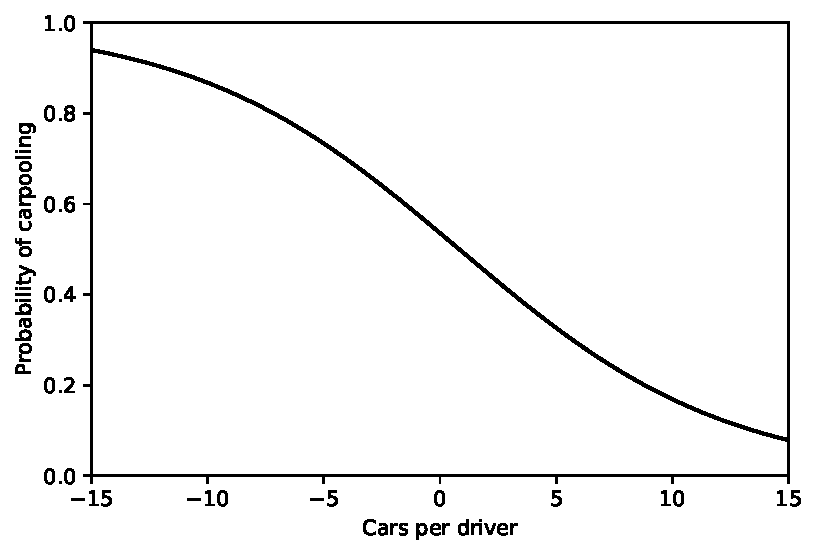
\includegraphics[width=\textwidth]{fig/logit.pdf}
    \end{column}
  \end{columns}
\end{frame}

\begin{frame}{The logit model}
  \centering\begin{tabular}{lrrrrrr}
  \toprule
  {} &  Coefficient &  Std. err. &  $t$-value &  $p$-value &  95\% Conf. &   Int. \\
  \midrule
  Constant        &        0.144 &      0.050 &      2.865 &      0.004 &      0.045 &  0.243 \\
  Cars per driver &       -0.174 &      0.039 &     -4.501 &      0.000 &     -0.250 & -0.098 \\
  \bottomrule
  \end{tabular}
  \begin{tabular}{lclc}
  Dependent variable & \multicolumn{3}{l}{Carpool on trip} \\
  Pseudo-$R^2$ & 0.00 & \\
  Sample size & 10000 && \\
  \end{tabular}\\
  \tiny\citenhts
\end{frame}

\begin{frame}{The logit model}
  \centering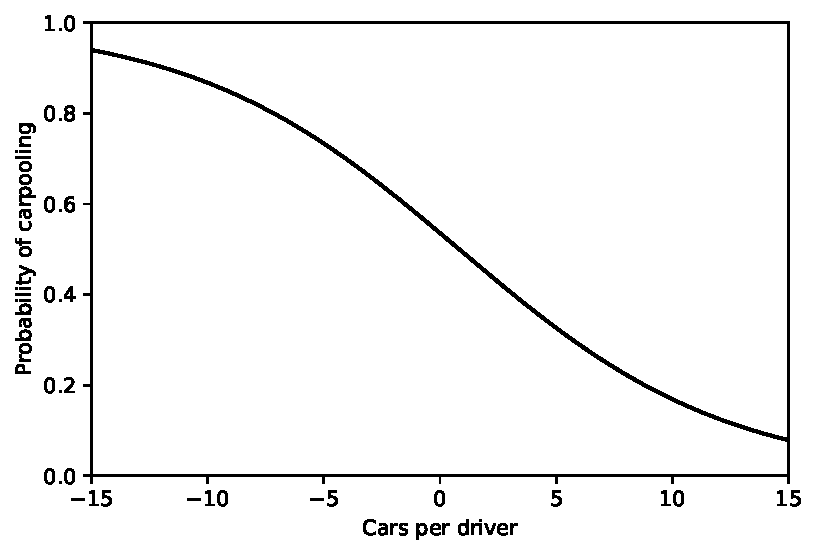
\includegraphics[width=0.65\textwidth]{fig/logit.pdf}\\
  \tiny\citenhts
\end{frame}

\begin{frame}{Interpreting the logit model: odds ratios}
  \begin{itemize}
    \item Coefficients in a logistic regression are hard to interpret
    \item Often presented as an \emph{odds ratio}, exponentiation of coefficient
    \item ...the ratio of the \emph{odds} of an event occurring when the variable increases by one
    \item Odds is the probability of the event divided by the probability of not the event
    \item For example, if the event occurs once and does not occur four times, the odds are one-to-four or $\frac{1}{4}$
    \pause\item ...what is the probability in this case?
  \end{itemize}
\end{frame}

\begin{frame}{Interpreting the logit model: odds ratios}
  \begin{itemize}
    \item Odds ratio greater than one, increase in outcome probability
    \item Odds ratio = 1, no relationship
    \item Odds ratio less than one, decrease in outcome probability
    \item The odds ratio is \textit{not} the ratio of probabilities, but is similar when the probability of the outcome is small
  \end{itemize}
\end{frame}

\begin{frame}{Logit model: example}
  \centering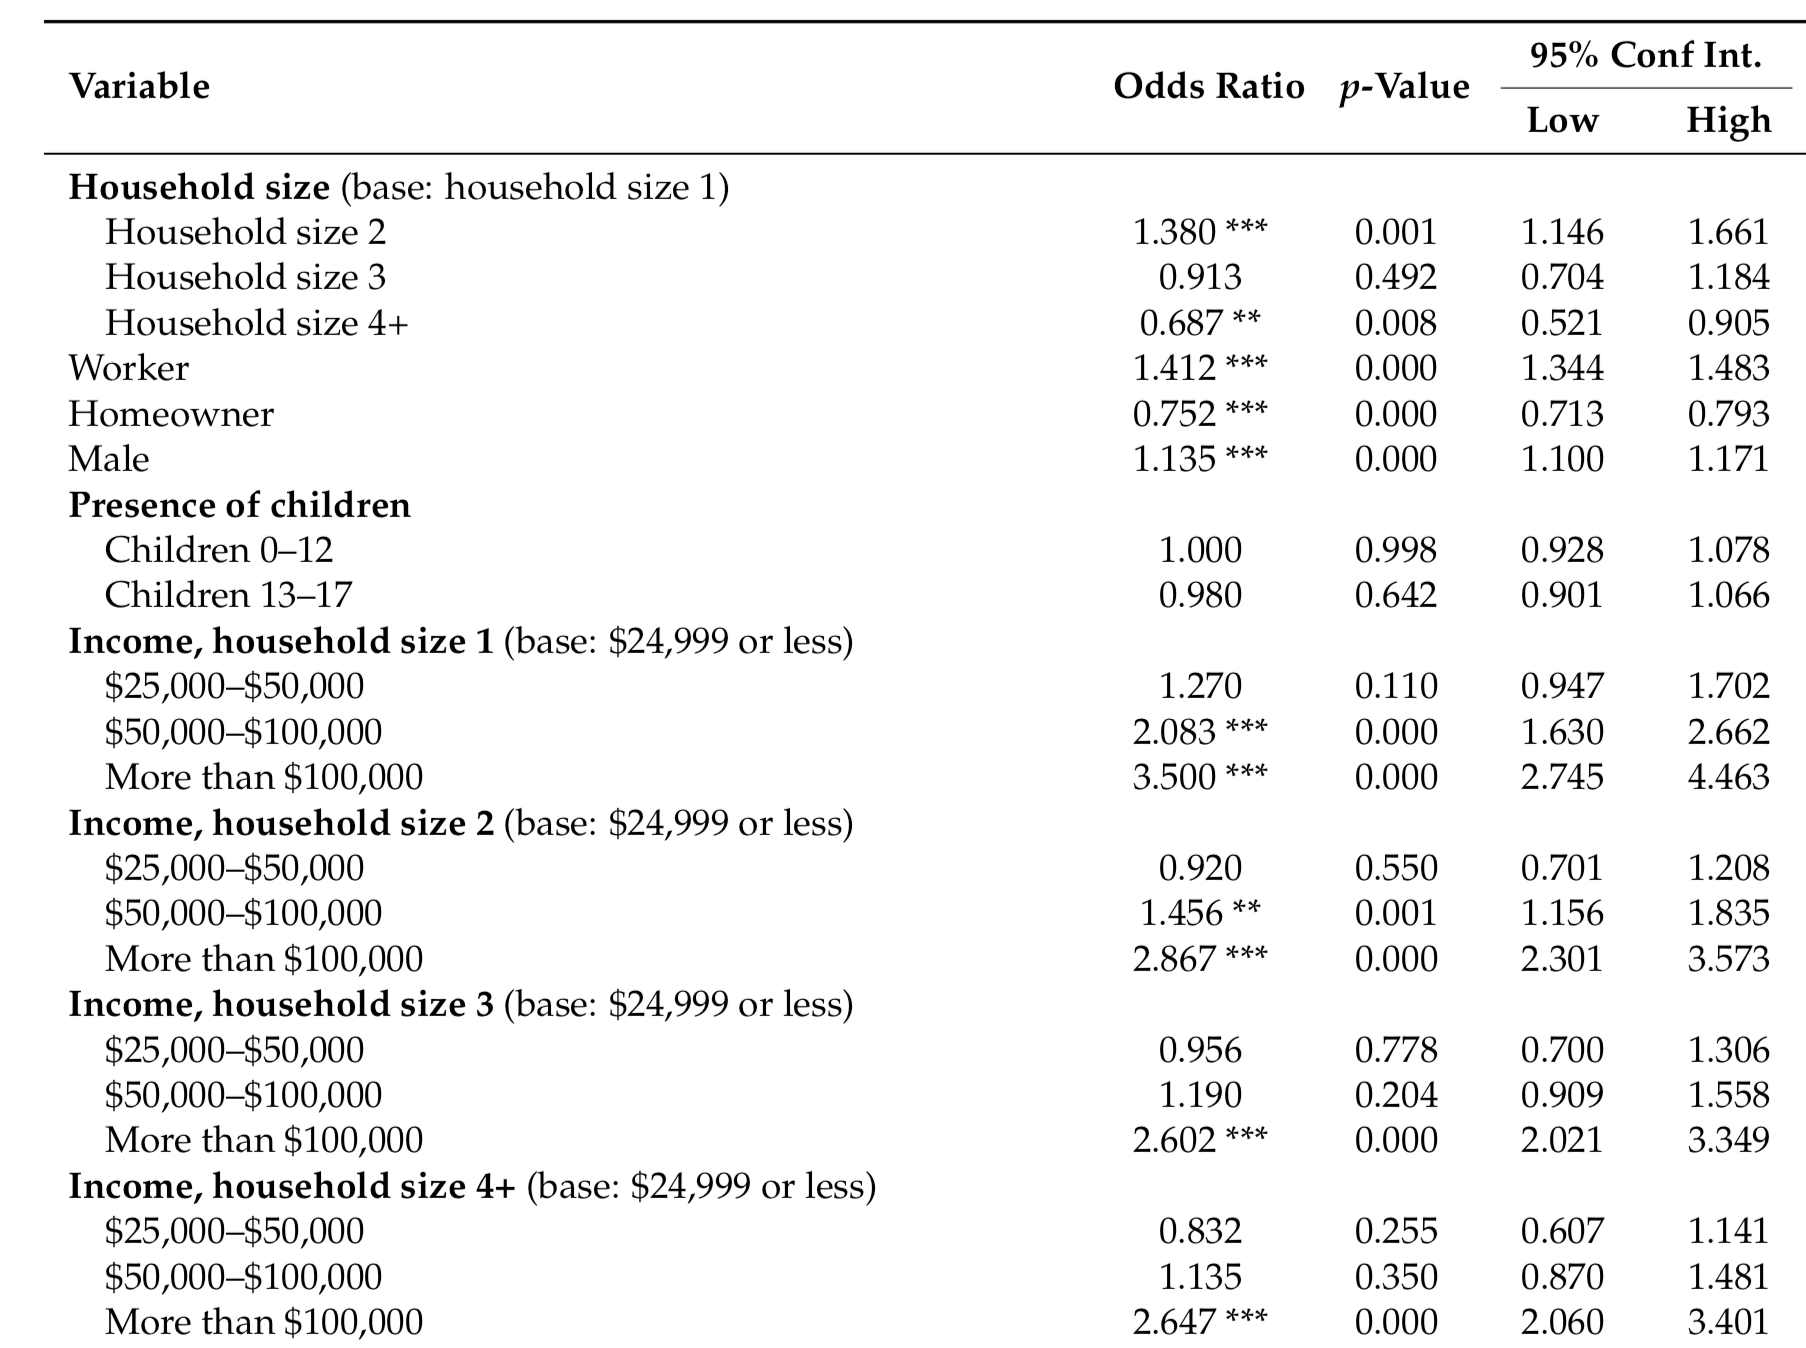
\includegraphics[width=0.6\textwidth]{fig/conway_logit.png}\\
  {\tiny \textcite{conway_trends_2018}}
\end{frame}

\begin{frame}{Logit model: example}
  \centering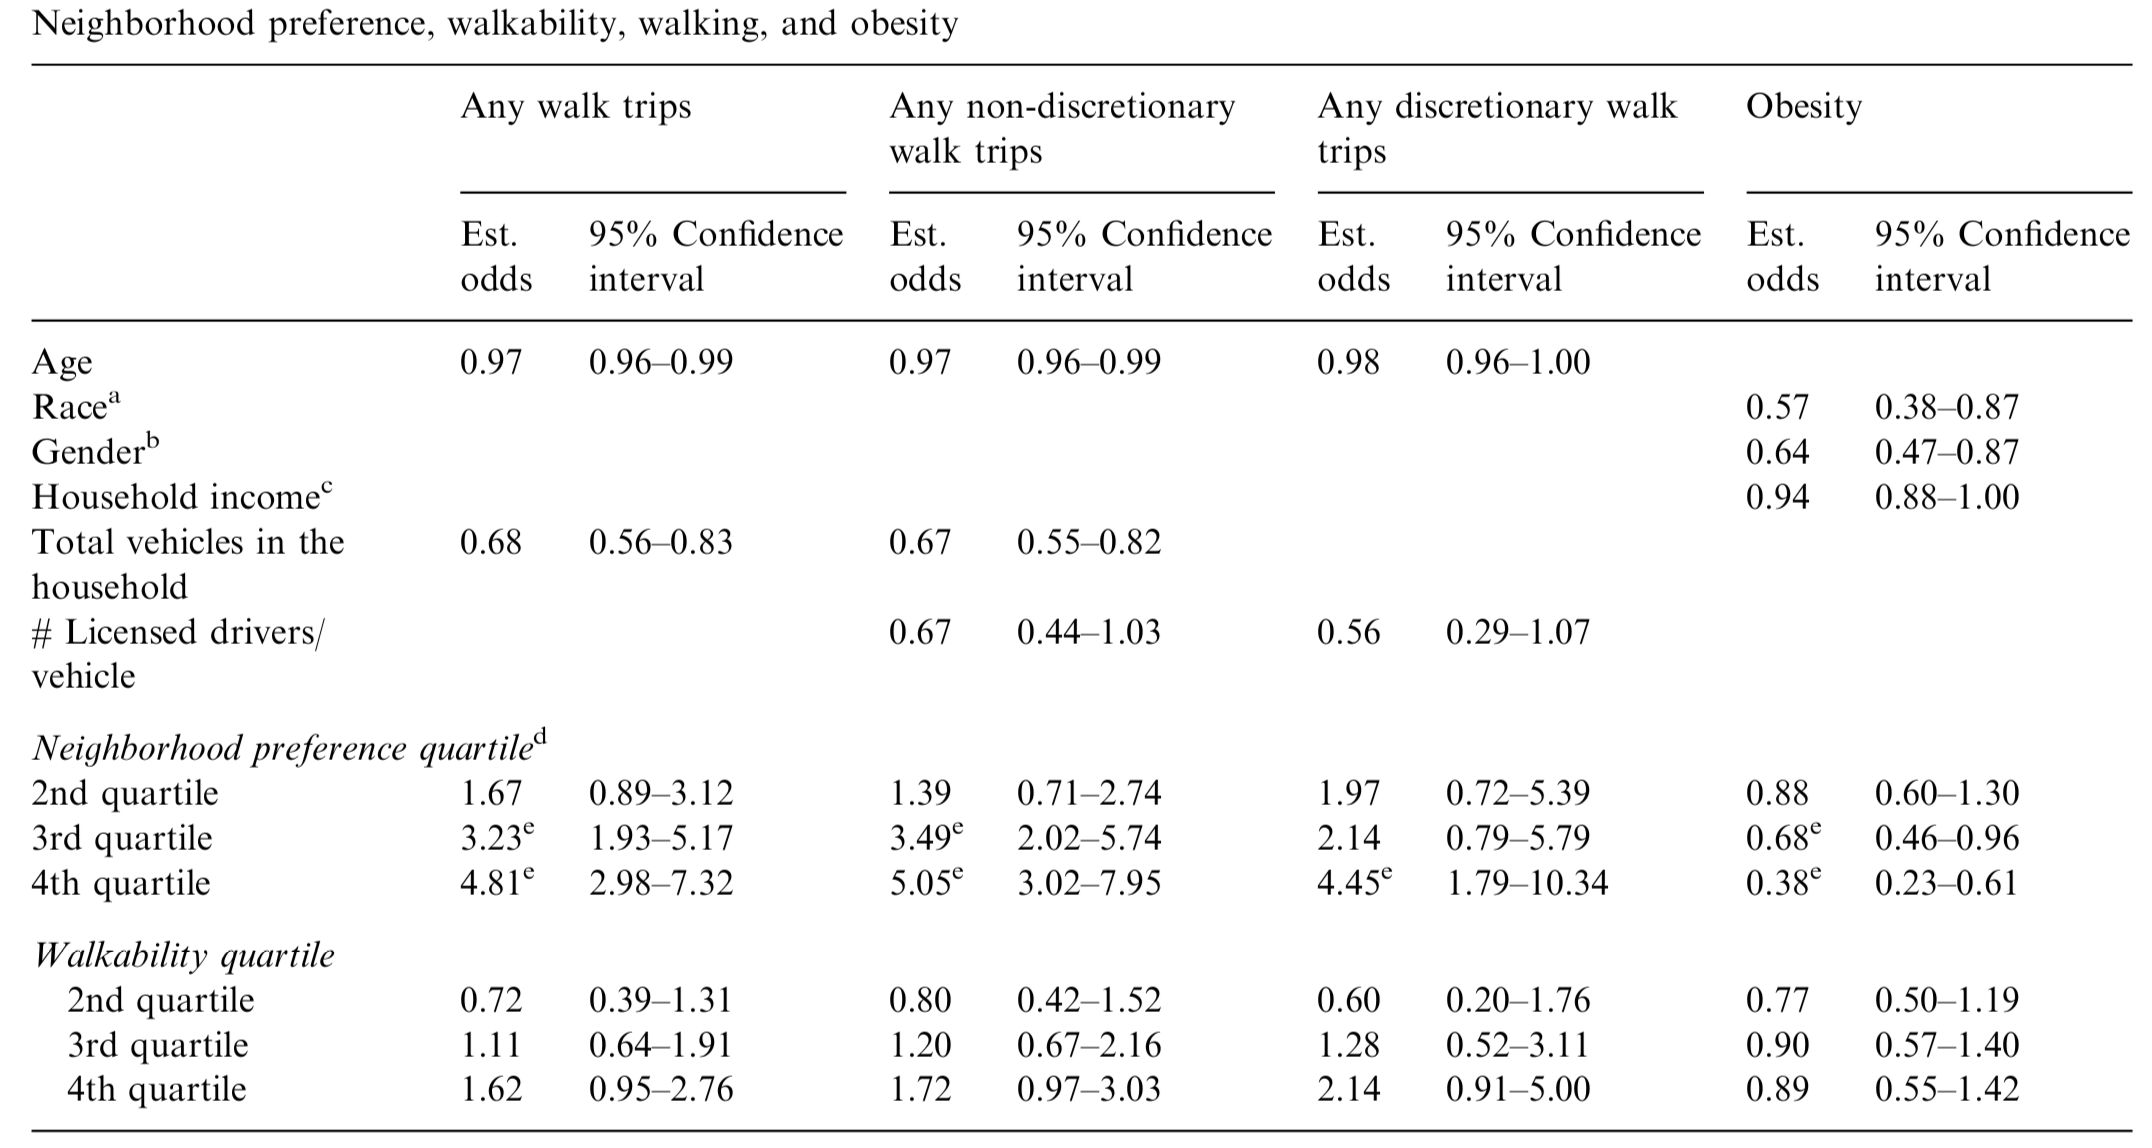
\includegraphics[width=0.8\textwidth]{fig/frank_logit.png}\\
  {\tiny \textcite{frank_stepping_2007}}
\end{frame}

\begin{frame}{Marginal effects}
  \begin{itemize}
    \item An alternate measure of the association between an independent and dependent variable is the \emph{marginal effect}
    \item This is the average amount the dependent variable changes for a unit change in the input variable
    \item In linear regression, this is the same as the coefficient
    \item But in other types of regression it isn't
    \item No need to record marginal effects unless coefficients/odds ratios are not reported
  \end{itemize}
\end{frame}

\begin{frame}{Other transformations: probit, tobit, etc.}
  \begin{itemize}
    \item There are a lot of other similar models with different transformation functions
    \item These represent different assumptions for the distribution of the random error term $\epsilon$
    \item Logit is by far the most common as the math is easier
  \end{itemize}
\end{frame}

\begin{frame}{More than two outcomes}
  \begin{columns}
    \begin{column}{0.65\textwidth}
      \begin{itemize}
        \item The logit models we've seen so far can only model two outcomes (e.g. carpool/not carpool)
        \item But what if we have more outcomes (e.g. bike/drive/walk)?
        \item In these cases we use a \emph{multinomial logit} model
      \end{itemize}
    \end{column}~%
    \begin{column}{0.34\textwidth}
      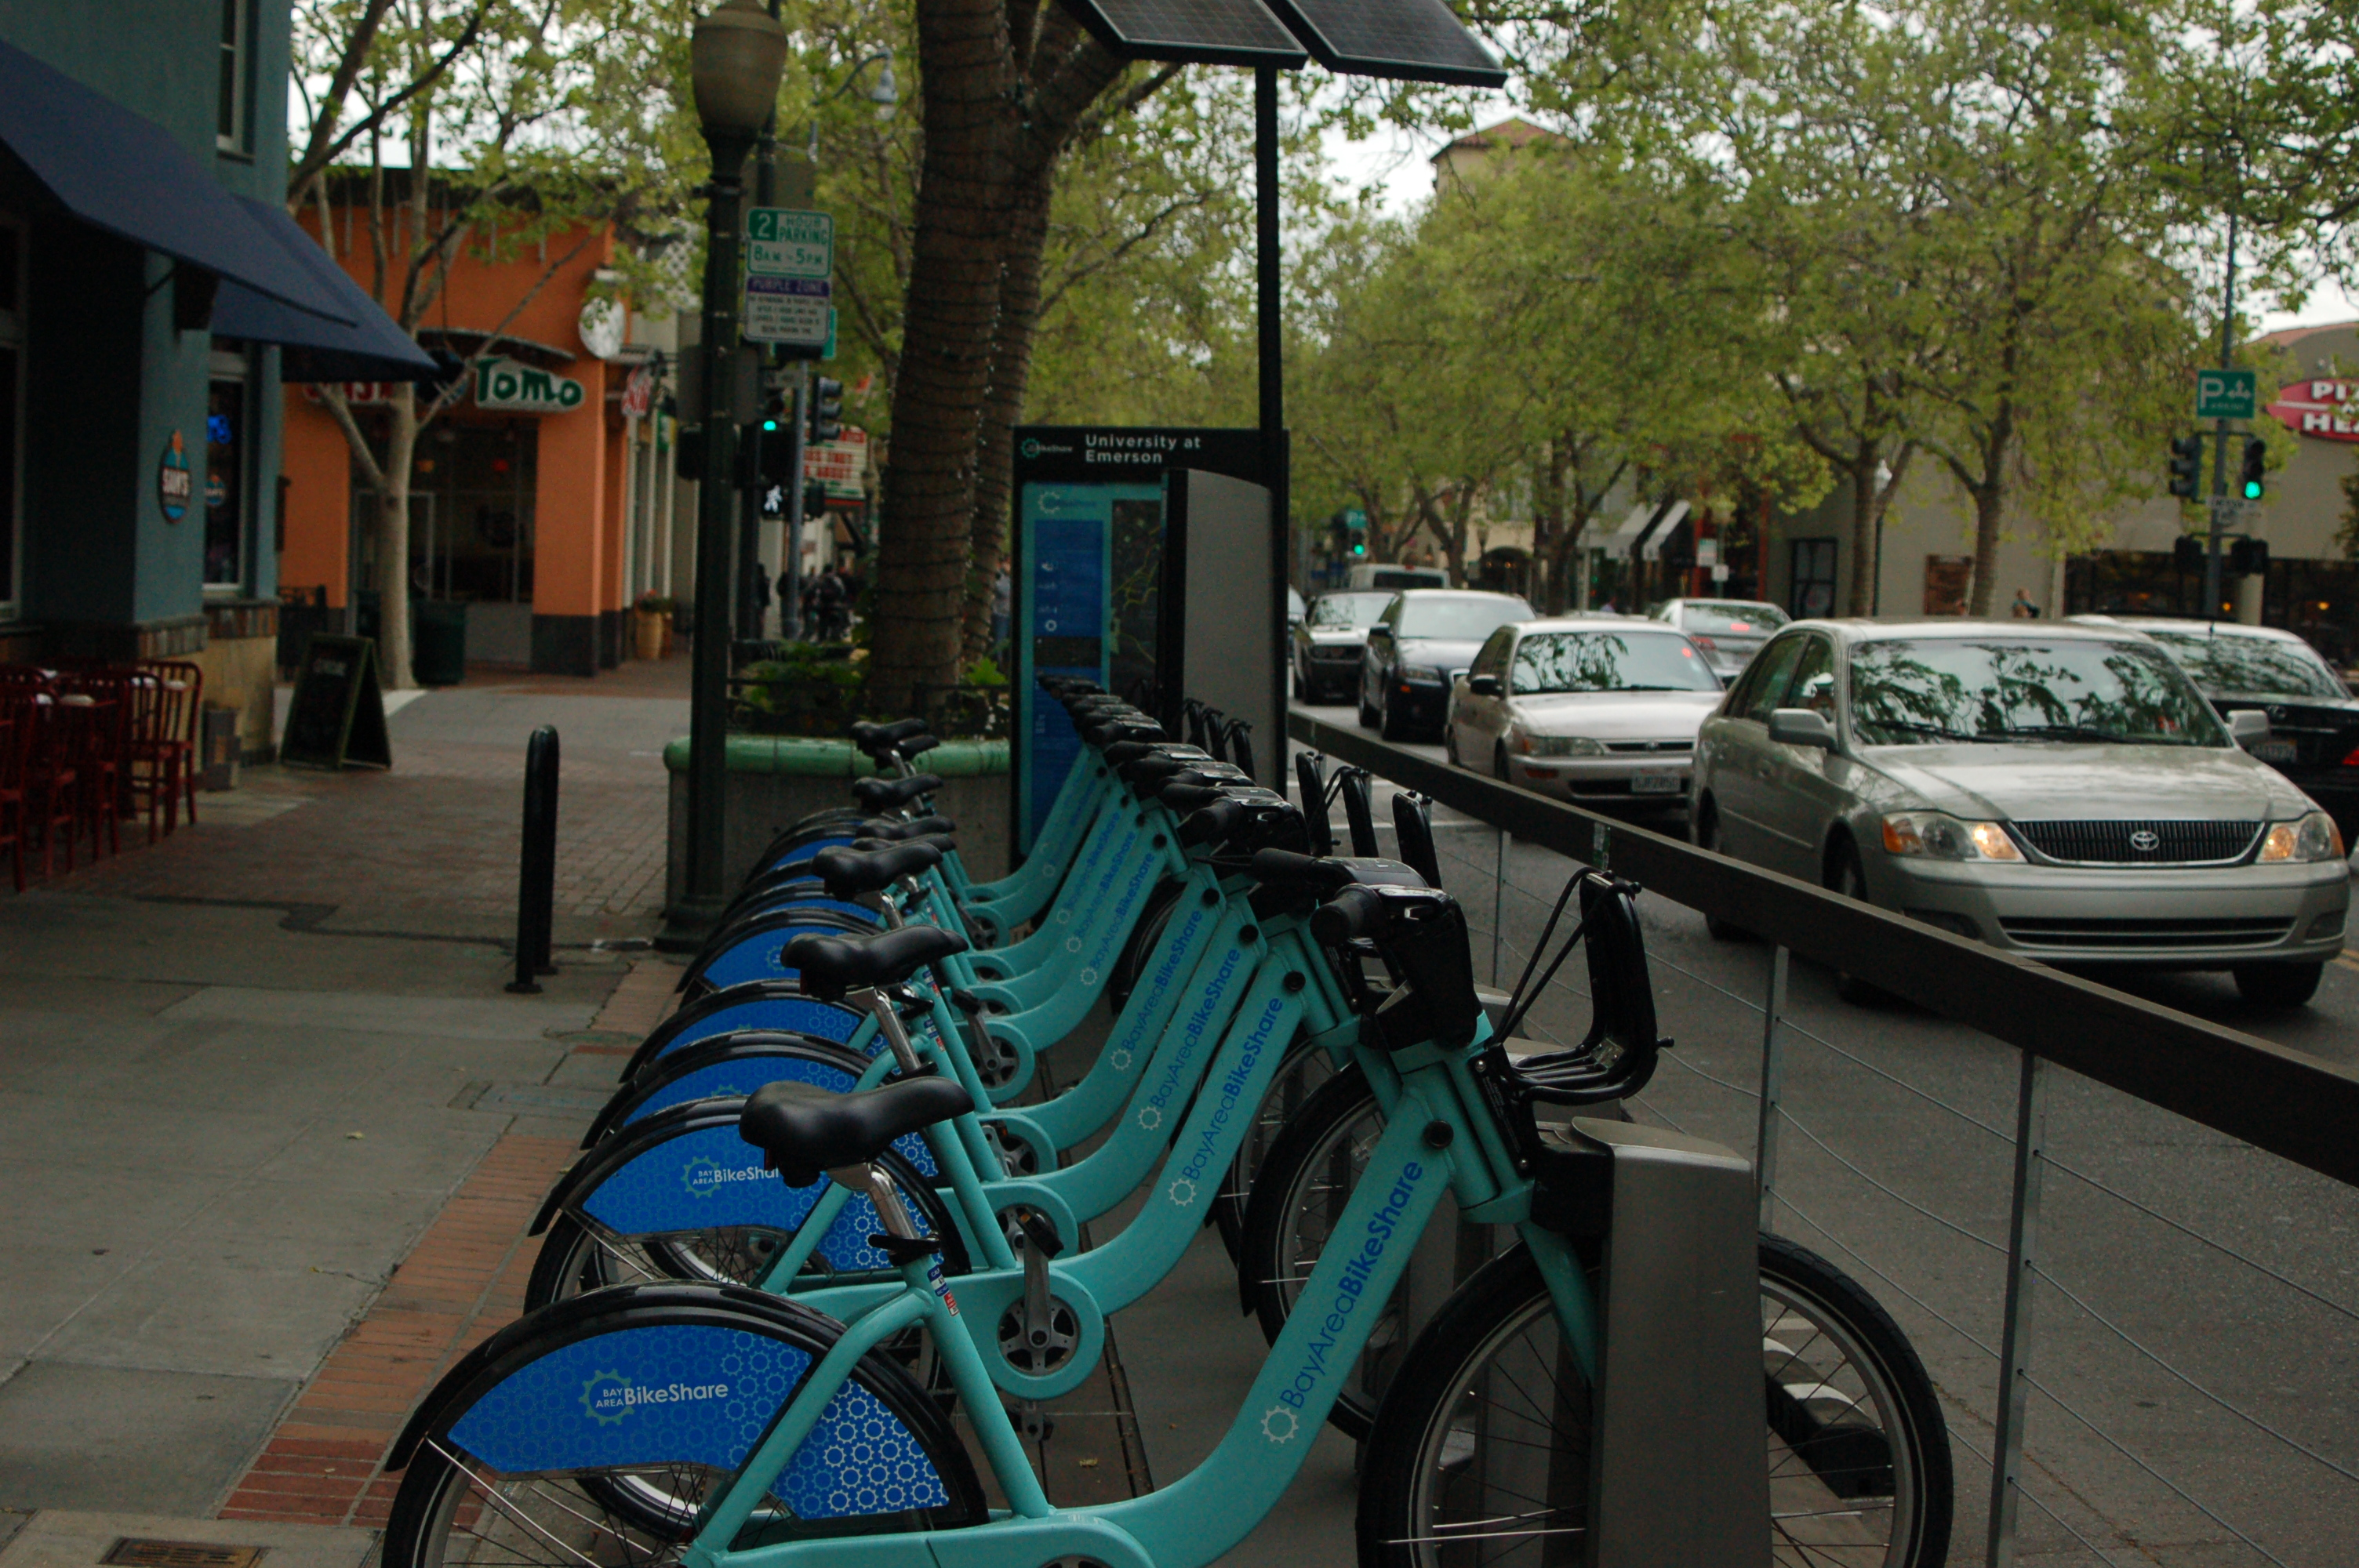
\includegraphics[width=\textwidth]{img/bikeshare.jpg}
    \end{column}
  \end{columns}
\end{frame}

\begin{frame}{The multinomial logit model}
  \begin{tikzpicture}
    \node[draw=black,inner sep=5pt,anchor=west] (inc) at (0, 4) { Income };
    \node[draw=black,inner sep=5pt,anchor=west] (ttwalk) at (0, 2) {Travel time by walk};
    \node[draw=black,inner sep=5pt,anchor=west] (ttpt) at (0, 1) {Travel time by transit};
    \node[draw=black,inner sep=5pt,anchor=west] (ttcar) at (0, 0) {Travel time by car};

    \node[draw=black,inner sep=5pt,anchor=west] (car) at (9, 2) { Probability of car };
    \node[draw=black,inner sep=5pt,anchor=west] (pt) at (9, 3) { Probability of transit };
    \node[draw=black,inner sep=5pt,anchor=west] (walk) at (9, 4) { Probability of walk };

    \pause
    \node[draw=black,inner sep=5pt,anchor=west,rounded corners=0.2cm] (ucar) at (5, 2) { Utility of car };
    \node[draw=black,inner sep=5pt,anchor=west,rounded corners=0.2cm] (upt) at (5, 3) { Utility of transit };
    \node[draw=black,inner sep=5pt,anchor=west,rounded corners=0.2cm] (uwalk) at (5, 4) { Utility of walk };

    \pause
    \draw[->] (inc.east) -- ([yshift=3pt]ucar.west) node[pos=0.2,outer sep=0,inner sep=0] (inccar) {};
    \draw[->] (inc.east) -- ([yshift=3pt]upt.west) node[pos=0.25,outer sep=0,inner sep=0] (incpt) {};
    \only<3-4>{\draw[->] (inc.east) -- ([yshift=3pt]uwalk.west) node[pos=0.23,outer sep=0,inner sep=0] (incwalk) {};}

    % \draw[->] (age.east) -- +(345:2.7cm) -- (ucar.west);
    % \draw[->] (age.east) -- (upt.west);
    % \draw[->] (age.east) -- (uwalk.west);

    \pause
    \only<4>{
    \node[text=red] (diff) at (2.5, 5) { Must be different! };

    \draw[draw=red,->] (diff.south) -- (inccar);
    \draw[draw=red,->] (diff.south) -- (incpt);
    \draw[draw=red,->] (diff.south) -- (incwalk);
    }

    \pause\pause
    \draw[->] (ttcar.east) -- ([yshift=-3pt]ucar.west) node[pos=0.2,outer sep=0,inner sep=0] (ttucar) {};
    \draw[->] (ttpt.east) -- ([yshift=-3pt]upt.west) node[pos=0.17,outer sep=0,inner sep=0] (ttupt) {};
    \draw[->] (ttwalk.east) -- ([yshift=-3pt]uwalk.west) node[pos=0.1,outer sep=0,inner sep=0] (ttuwalk) {};

    \pause
    \node[text=red] (same) at (5, 0) { Can be same };

    \draw[draw=red,->] (same.north) -- (ttucar);
    \draw[draw=red,->] (same.north) -- (ttuwalk);
    \draw[draw=red,->] (same.north) -- (ttupt);

    \pause

    \draw[->] (ucar.east) -- ([yshift=-3pt]car.west);
    \draw[->] (upt.east) -- (pt.west);
    \draw[->] (uwalk.east) -- ([yshift=3pt]walk.west);

    \pause

    \draw[->,draw=black!40] (ucar.east) -- ([yshift=-3pt]pt.west);
    \draw[->,draw=black!40] (ucar.east) -- ([yshift=-3pt]walk.west);
    \draw[->,draw=black!40] (upt.east) -- (car.west);
    \draw[->,draw=black!40] (upt.east) -- (walk.west);
    \draw[->,draw=black!40] (uwalk.east) -- ([yshift=3pt]car.west);
    \draw[->,draw=black!40] (uwalk.east) -- ([yshift=3pt]pt.west);

    \pause
    \draw[<-] (uwalk.north) -- +(90:0.5cm) node[text=black,anchor=south] {$\epsilon$};
    \draw[<-] ([xshift=1em] ucar.south) -- +(270:0.5cm) node[text=black,anchor=north] {$\epsilon$};
    \draw[<-] ([xshift=3em]upt.south) -- +(270:1.5cm) node[text=black,anchor=north] {$\epsilon$};
  \end{tikzpicture}
\end{frame}

\begin{frame}{Multinomial logit model: mathematical form}
  \begin{tabular}{lllll}
    $U_{walk}$ & $= \only<1>{\alpha_{walk}}$ & $\only<1>{+ \beta_{income,walk} x_{income}}$ & $\only<1>{+} \beta_{time} x_{time,walk}$ & $+ \epsilon_{walk}$ \\
    \\
    $U_{transit}$ & $= \alpha_{transit}$ & $+ \beta_{income,transit} x_{income}$ & $+ \beta_{time} x_{time,transit}$ & $+ \epsilon_{transit}$ \\
    \\
    $U_{car}$ & $= \alpha_{car}$ & $+ \beta_{income,car} x_{income}$ & $+ \beta_{time} x_{time,car}$ & $+ \epsilon_{car}$ \\
  \end{tabular}

  \pause
  \pause
  \vspace{2em}
  $p_{walk} = \frac{e^{U_{walk}}}{\sum_{m \in \{walk, transit, car\}}e^{U_m}}$
\end{frame}

\begin{frame}{Multinomial logit model: results}
  \centering\begin{tabular}{lrrrrrrr}
\toprule
{} &  Value &  Std err &  t-test &  p-value  \\
\midrule
  \textbf{Car} \\
  \hspace*{1em} Alternative specific constant &   1.58 &     0.37 &    4.31 &      0.0  \\
  \hspace*{1em} Income (thousands CHF/month)   &  -0.15 &     0.04 &   -3.42 &      0.0  \\
  \textbf{Transit} \\
  \hspace*{1em} Alternative specific constant      &   1.36 &     0.37 &    3.65 &      0.0 \\
  \hspace*{1em} Income (thousands CHF/month)      &  -0.16 &     0.05 &   -3.46 &      0.0 \\
  Travel time &  -0.01 &     0.00 &  -11.77 &      0.0 \\
  \bottomrule
\end{tabular}\\
{\tiny Data: \textcite{bierlaire_mode_2018}}
\end{frame}

\begin{frame}{Multinomial logit model: example}
  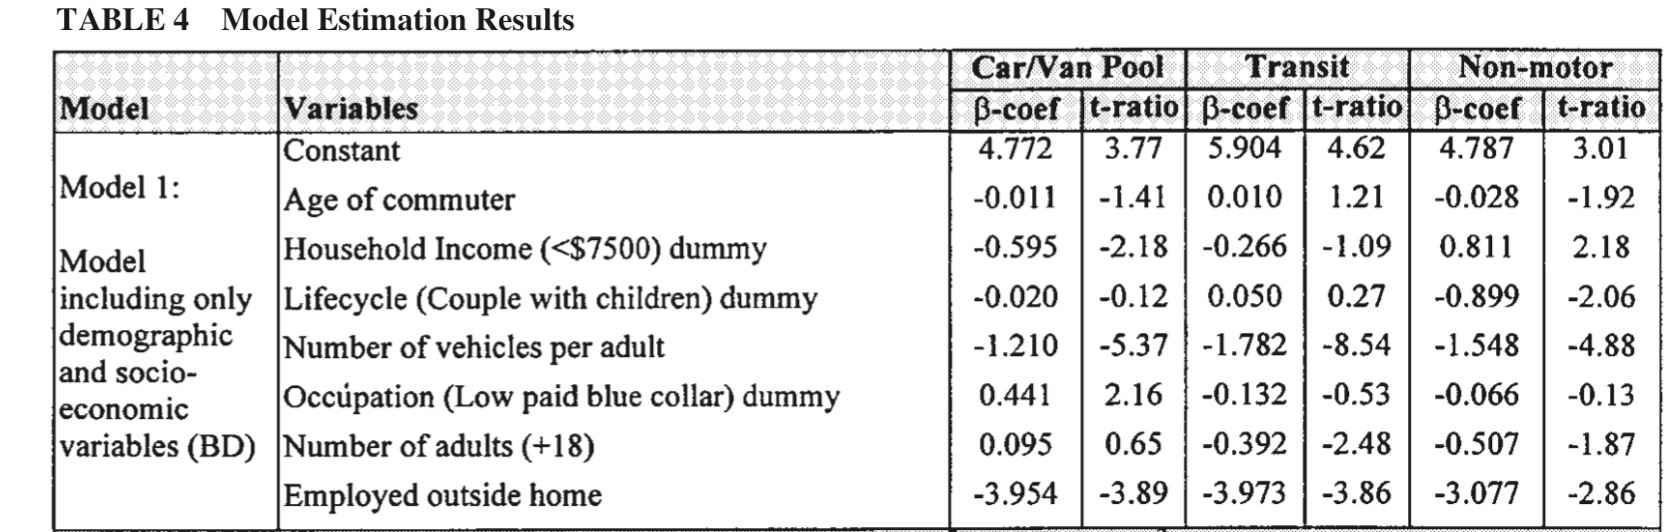
\includegraphics[width=\textwidth]{img/kuppam.png}\\
  {\tiny \textcite{kuppam_analysis_1999}}
\end{frame}
